
\section*{TP 9 : Rotation et vibration des molécules diatomiques}
\begin{itemize}
	
	\item Vibration de molécules diatomiques
		\begin{itemize}
			
			\item Approximation parabolique 
				\begin{equation}
				V = \frac{1}{2}\mu \omega ^2 (R-R_0)^2
				\end{equation}
					
			\item Energie de vibration valable à courtes distances 
				\begin{equation}
				E_{n,vib} = (n+\frac{1}{2})\hbar \omega
				\end{equation}
			\end{itemize}
		
		\item Rotation de molécules diatomiques
			
			\begin{itemize}
				\item Hamiltonien de rotation
					\begin{equation}
					H_{rot} = \frac{L^2}{2I} \qquad \Rightarrow \qquad E_{l,rot} = \frac{\hbar ^2 l(l+1)}{2I} \qquad avec \ I = \mu r_0 ^2
					\end{equation}
				
				\item Classification des différentes énergies
					\begin{equation}
					E_{rot} < E_{vib} < Ryd
					\end{equation}
			\end{itemize}
			
		\item Transition dipolaire électrique $\Delta l = 1$

			\begin{itemize}
				\item Absorption : $l_f = l_i + 1$
				\item Emission : $l_f = l_i - 1$
				\item Les raies d'absorption et d'émission correspondent aux énergies de transition admises
			\end{itemize}
\end{itemize}

\begin{figure}[h]
	\begin{center}
		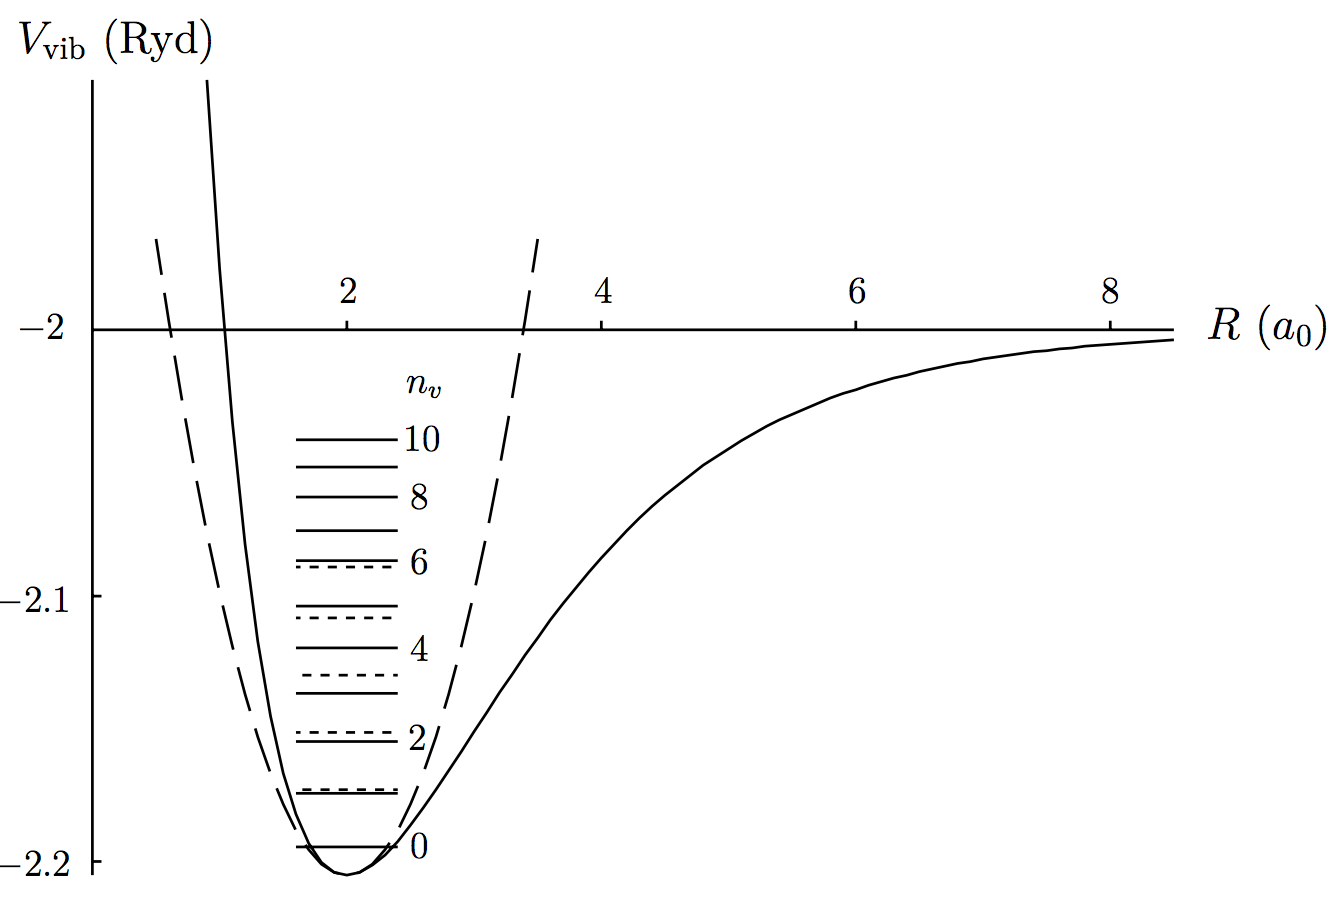
\includegraphics[scale=0.5]{1}
		\caption{Spectre de vibration de la molécule $H_2$.}
	\end{center}
\end{figure}